\section{Implementación}
\setcounter{sectiontotal}{11}

\iflinux
    \newenvironment{step}[2]%
{%
% Workaroudn terrible http://tex.stackexchange.com/questions/17036/why-cant-the-end-code-of-an-environment-contain-an-argument
\def\fooNoA{#1}
\def\fooNoB{#2}

%Primer frame
\begin{frame}[noframenumbering]%
\frametitle{\pagetitle}%
\framesubtitle{#1 (1 de 2)}%
%\begin{itemize}%
}%
{%
%\end{itemize}%
\end{frame}%

%Segundo frame
\begin{frame}[noframenumbering]%
\frametitle{\pagetitle}%
\framesubtitle{\fooNoA{}~(2 de 2)}%
\movie[%
height=0.7\textheight,%
width=\textwidth,%
showcontrols,%
poster,%
autostart%
]{}{\fooNoB}%
\end{frame}%
}


\else
    \newenvironment{step}[2]%
{%
% Workaroudn terrible http://tex.stackexchange.com/questions/17036/why-cant-the-end-code-of-an-environment-contain-an-argument
\def\fooNoA{#1}
\def\fooNoB{#2}

%Primer frame
\begin{frame}%
\frametitle{\pagetitle}%
\framesubtitle{#1 (1 de 2)}%
%\begin{itemize}%
}%
{%
%\end{itemize}%
\end{frame}%

%Segundo frame
\begin{frame}[noframenumbering]%
\frametitle{\pagetitle}%
\framesubtitle{\fooNoA{}~(2 de 2)}%
\includemedia[
  height=0.7\textheight,%
  width=\textwidth,%
  activate=pageopen,%
  deactivate=pageclose,%
  addresource=\fooNoB,
  flashvars={source=\fooNoB}
]{}{VPlayer.swf}
\end{frame}%
}


\fi

\begin{frame}
\frametitle{\pagetitle}
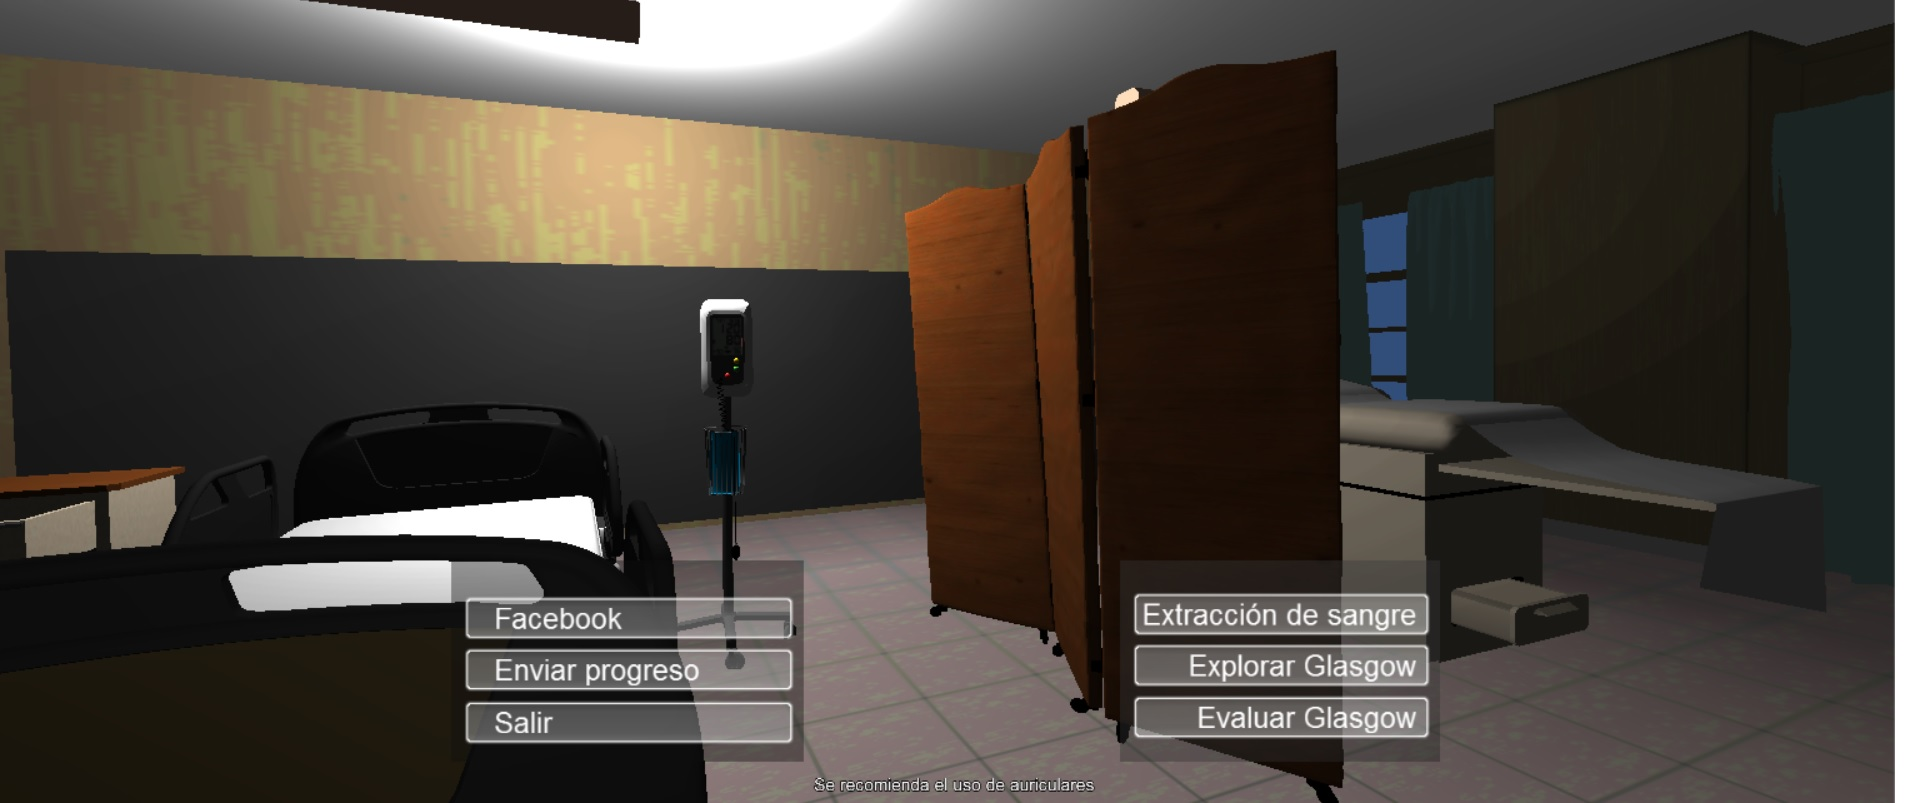
\includegraphics[width=\textwidth]{../solucion/images/pantalla_inicio.jpg}%
\end{frame}

\begin{step}{Inicio}{videos/inicio_1.mp4}
\begin{itemize}
    \item Visión del laboratorio
    \item Envió de datos
\end{itemize}
\end{step}

\begin{step}{Venopunción Inicio}{./videos/veno_1_movimientos.mp4}
\begin{itemize}
    \item Mover la cámara
    \item Acercar/alejar
\end{itemize}
\end{step}

\begin{step}{Venopunción Paciente}{./videos/veno_2_entorno.mp4}
\begin{itemize}
    \item Reacción del paciente
    \item Sentir el pulso
    \item Interacción verbal
\end{itemize}
\end{step}

\begin{step}{Venopunción Opciones}{./videos/veno_3_opciones.mp4}
\begin{itemize}
    \item Opciones de bioseguridad
    \item Estado del usuario
\end{itemize}
\end{step}

\begin{step}{Venopunción Elementos}{./videos/veno_4_elementos.mp4}
\begin{itemize}
    \item Utilización de elementos
    \item Extracción de sangre
\end{itemize}
\end{step}


\begin{step}{Venopunción Evaluación}{./videos/veno_5_resultados.mp4}
\begin{itemize}
    \item Utilización de un motor de reglas
    \item Evaluación dependiente del contexto
\end{itemize}
\end{step}


\begin{step}{Glasgow Exploración}{./videos/glasgow_1_seleccion_estado.mp4}
\begin{itemize}
    \item Posibilidad de interactuar con un paciente con el estado deseado
\end{itemize}
\end{step}

\begin{step}{Glasgow Reacción}{./videos/glasgow_2_interaccion.mp4}
\begin{itemize}
    \item Interactuar con un paciente a través del habla.
    \item Reacciones oculares.
    \item Reacciones motoras
    \item Reacciones verbales
\end{itemize}
\end{step}


\begin{step}{Glasgow Reacción}{./videos/glasgow_3_full.mp4}
\begin{itemize}
    \item Flujo completo del análisis.
    \item Evaluación del paciente.
    \item Evaluación al alumno.
\end{itemize}
\end{step}

\begin{frame}
\frametitle{\pagetitle}
\framesubtitle{Componentes}
\begin{figure}
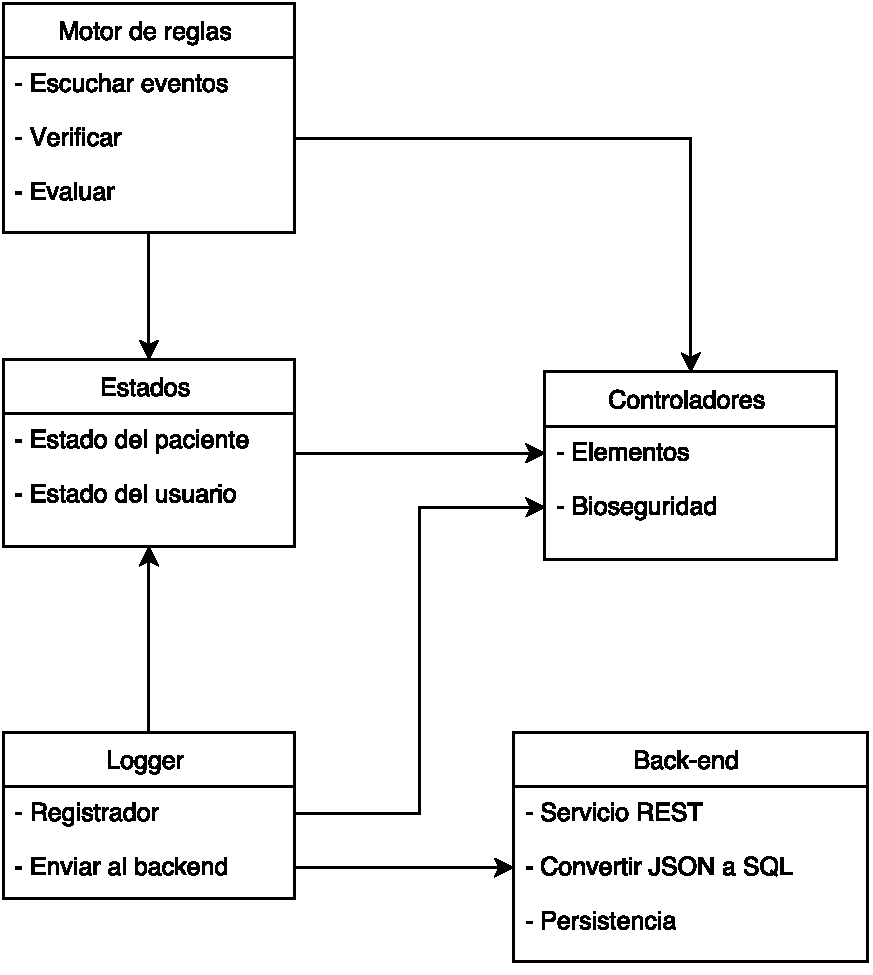
\includegraphics[width=\textwidth,height=0.75\textheight,keepaspectratio]{./imagenes/esquema_global.pdf}
\end{figure}
\end{frame}
